\documentclass[tikz,border=8pt]{standalone}
% Shared look for every TikZ diagram. Load with % Shared look for every TikZ diagram. Load with % Shared look for every TikZ diagram. Load with \input{../../tools/tikz-style.tex}
\usepackage[T1]{fontenc}
\usepackage{lmodern}
\renewcommand{\sfdefault}{lmr}  % diagrams use the same serif as the text
\usetikzlibrary{arrows.meta, positioning, shapes.geometric, calc, fit, backgrounds}
\definecolor{cblue}{HTML}{4C78A8}
\definecolor{corange}{HTML}{F58518}
\definecolor{cgreen}{HTML}{54A24B}
\definecolor{cred}{HTML}{E45756}
\definecolor{cpurple}{HTML}{B279A2}
\definecolor{cgrey}{HTML}{6B6B6B}
\tikzset{
  every picture/.style={font=\sffamily, line width=1.2pt},
  box/.style={draw=#1, fill=#1!12, rounded corners=4pt, align=center, inner sep=7pt, minimum height=1.1cm},
  box/.default=cgrey,
  arrow/.style={-{Stealth[length=3mm]}, draw=cgrey, line width=1.4pt},
  title/.style={font=\sffamily\bfseries\Large},
  note/.style={font=\sffamily\small, text=cgrey, align=center},
}
\AtBeginDocument{\hyphenpenalty=10000 \exhyphenpenalty=10000}

\usepackage[T1]{fontenc}
\usepackage{lmodern}
\renewcommand{\sfdefault}{lmr}  % diagrams use the same serif as the text
\usetikzlibrary{arrows.meta, positioning, shapes.geometric, calc, fit, backgrounds}
\definecolor{cblue}{HTML}{4C78A8}
\definecolor{corange}{HTML}{F58518}
\definecolor{cgreen}{HTML}{54A24B}
\definecolor{cred}{HTML}{E45756}
\definecolor{cpurple}{HTML}{B279A2}
\definecolor{cgrey}{HTML}{6B6B6B}
\tikzset{
  every picture/.style={font=\sffamily, line width=1.2pt},
  box/.style={draw=#1, fill=#1!12, rounded corners=4pt, align=center, inner sep=7pt, minimum height=1.1cm},
  box/.default=cgrey,
  arrow/.style={-{Stealth[length=3mm]}, draw=cgrey, line width=1.4pt},
  title/.style={font=\sffamily\bfseries\Large},
  note/.style={font=\sffamily\small, text=cgrey, align=center},
}
\AtBeginDocument{\hyphenpenalty=10000 \exhyphenpenalty=10000}

\usepackage[T1]{fontenc}
\usepackage{lmodern}
\renewcommand{\sfdefault}{lmr}  % diagrams use the same serif as the text
\usetikzlibrary{arrows.meta, positioning, shapes.geometric, calc, fit, backgrounds}
\definecolor{cblue}{HTML}{4C78A8}
\definecolor{corange}{HTML}{F58518}
\definecolor{cgreen}{HTML}{54A24B}
\definecolor{cred}{HTML}{E45756}
\definecolor{cpurple}{HTML}{B279A2}
\definecolor{cgrey}{HTML}{6B6B6B}
\tikzset{
  every picture/.style={font=\sffamily, line width=1.2pt},
  box/.style={draw=#1, fill=#1!12, rounded corners=4pt, align=center, inner sep=7pt, minimum height=1.1cm},
  box/.default=cgrey,
  arrow/.style={-{Stealth[length=3mm]}, draw=cgrey, line width=1.4pt},
  title/.style={font=\sffamily\bfseries\Large},
  note/.style={font=\sffamily\small, text=cgrey, align=center},
}
\AtBeginDocument{\hyphenpenalty=10000 \exhyphenpenalty=10000}

\begin{document}
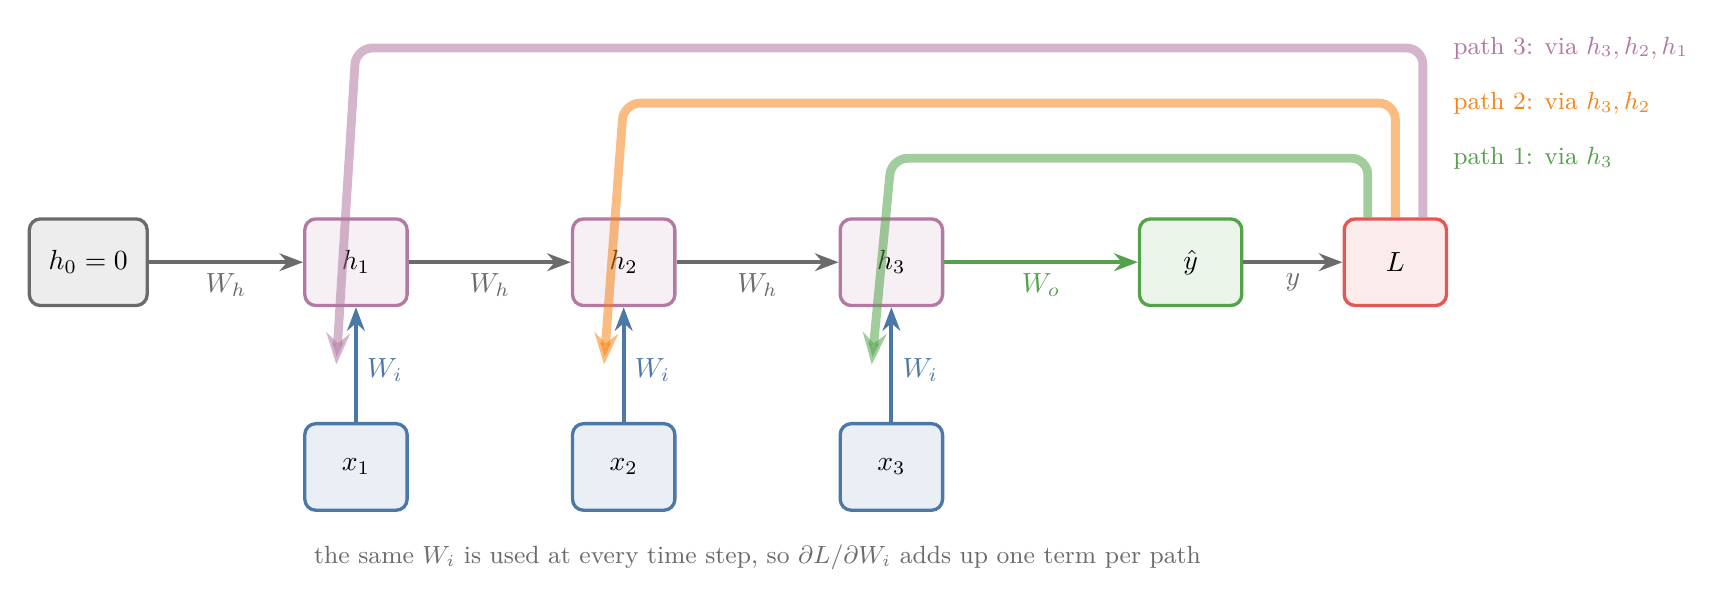
\begin{tikzpicture}[st/.style={box=cpurple, minimum width=1.3cm}, inp/.style={box=cblue, minimum width=1.3cm},
  bp/.style={line width=3.2pt, opacity=0.55, -{Stealth[length=4mm]}, rounded corners=6pt}]
  \node[box=cgrey, minimum width=1.3cm] (h0) at (0,0) {$h_0 = 0$};
  \foreach \t in {1,2,3} {
    \node[st] (h\t) at (3.4*\t,0) {$h_\t$};
    \node[inp] (x\t) at (3.4*\t,-2.6) {$x_\t$};
    \draw[arrow, draw=cblue] (x\t) -- node[right, text=cblue, pos=0.45] {$W_i$} (h\t);
  }
  \draw[arrow] (h0) -- node[below, text=cgrey] {$W_h$} (h1);
  \draw[arrow] (h1) -- node[below, text=cgrey] {$W_h$} (h2);
  \draw[arrow] (h2) -- node[below, text=cgrey] {$W_h$} (h3);
  \node[box=cgreen, minimum width=1.3cm] (y) at (14.0,0) {$\hat{y}$};
  \node[box=cred, minimum width=1.3cm] (L) at (16.6,0) {$L$};
  \draw[arrow, draw=cgreen] (h3) -- node[below, text=cgreen] {$W_o$} (y);
  \draw[arrow] (y) -- node[below, text=cgrey] {$y$} (L);
  % backward paths from L to each use of W_i
  \draw[bp, cgreen] ([xshift=-0.35cm]L.north) -- ([xshift=-0.35cm, yshift=0.75cm]L.north) -- ([yshift=0.75cm]L.north -| h3) -- ([xshift=-0.25cm]$(x3)!0.5!(h3)$);
  \draw[bp, corange] ([xshift=0cm]L.north) -- ([xshift=0cm, yshift=1.45cm]L.north) -- ([yshift=1.45cm]L.north -| h2) -- ([xshift=-0.25cm]$(x2)!0.5!(h2)$);
  \draw[bp, cpurple] ([xshift=0.35cm]L.north) -- ([xshift=0.35cm, yshift=2.15cm]L.north) -- ([yshift=2.15cm]L.north -| h1) -- ([xshift=-0.25cm]$(x1)!0.5!(h1)$);
  \node[note, text=cgreen, anchor=west] at ([xshift=0.6cm, yshift=0.75cm]L.north) {path 1: via $h_3$};
  \node[note, text=corange, anchor=west] at ([xshift=0.6cm, yshift=1.45cm]L.north) {path 2: via $h_3, h_2$};
  \node[note, text=cpurple, anchor=west] at ([xshift=0.6cm, yshift=2.15cm]L.north) {path 3: via $h_3, h_2, h_1$};
  \node[note] at (8.5,-3.75) {the same $W_i$ is used at every time step, so $\partial L/\partial W_i$ adds up one term per path};
\end{tikzpicture}
\end{document}
